\documentclass{standalone}
\usepackage{tikz}
\begin{document}
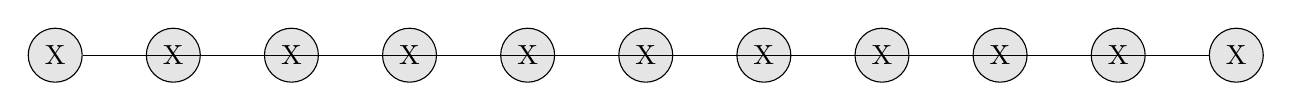
\begin{tikzpicture}[scale=1]
\node[draw,circle,fill=gray!20] (v0) at (0,0) {X};
\node[draw,circle,fill=gray!20] (v7) at (1.5,0) {X};
\node[draw,circle,fill=gray!20] (v3) at (3,0) {X};
\node[draw,circle,fill=gray!20] (v10) at (4.5,0) {X};
\node[draw,circle,fill=gray!20] (v6) at (6,0) {X};
\node[draw,circle,fill=gray!20] (v2) at (7.5,0) {X};
\node[draw,circle,fill=gray!20] (v9) at (9,0) {X};
\node[draw,circle,fill=gray!20] (v5) at (10.5,0) {X};
\node[draw,circle,fill=gray!20] (v1) at (12,0) {X};
\node[draw,circle,fill=gray!20] (v8) at (13.5,0) {X};
\node[draw,circle,fill=gray!20] (v4) at (15,0) {X};
\draw (v0) -- (v1);
\draw (v7) -- (v8);
\draw (v3) -- (v4);
\draw (v6) -- (v7);
\draw (v2) -- (v3);
\draw (v9) -- (v10);
\draw (v5) -- (v6);
\draw (v1) -- (v2);
\draw (v8) -- (v9);
\draw (v4) -- (v5);
\end{tikzpicture}
\end{document}
